\documentclass[
    11pt,
    spanish,
	a4paper
]{article}
\usepackage[utf8]{inputenc}
\usepackage[spanish]{babel}
\usepackage{graphicx}
\usepackage{authoraftertitle}
\usepackage{float}
\usepackage{caption}
\usepackage{verbatim}
\usepackage{listings}
\captionsetup[table]{labelformat=empty}

\def\doctype{Trabajo práctico}
\title{Simulaciones}
\author{Gonzalo Nahuel Vaca}

\begin{document}

\makeatletter
\begin{titlepage}
	\begin{center}
		\vspace*{1cm}
		
		\Huge
		\textbf{\doctype}
		\vspace{0.5cm}
    
		\LARGE
		\@title
		\vspace{0.5cm}
    
		\textbf{Compatibilidad Electromagnética}
		
		\vspace{1.5cm}
		
		\textbf{\@author}

		\vspace{1.5cm}

		
\includegraphics[width=0.8\textwidth]{../img/logoFIUBA.pdf}
		
		\vfill
		Departamento de Ingeniería e Investigaciones Tecnológicas\\
		Universidad Nacional de la Matanza\\
		Argentina\\
		\today
	\end{center}
\end{titlepage}
\makeatother
\newpage

\section{Código fuente}

\begin{lstlisting}
import numpy as np
import matplotlib.pyplot as plt
from scipy import signal

def senoidal(fs: "Hz", fo: "Hz", amp: "[0,1]",
             muestras: int, fase: "rad"):
    dominio = np.arange(muestras)
    imagen = amp * np.sin(
      (2 * np.pi * fs * dominio / fo) + fase)
    return (imagen + amp) / 2


def triangular(fs: "Hz", fo: "Hz", amp: "[0,1]",
               muestras: int, fase: "rad"):
    forma_triangulo = 0.5
    dominio = np.arange(muestras)
    imagen = amp * signal.sawtooth((2 * np.pi *
             fs * dominio / fo) + fase, forma_triangulo)
    return (imagen + amp)/2


def cuadrada(fs: "Hz", fo: "Hz", amp: "[0,1]",
             muestras: int, fase: "rad"):
    forma_cuadrada = 0.5
    dominio = np.arange(muestras)
    imagen = amp * signal.square((2 * np.pi * fs *
             dominio / fo) + fase, forma_cuadrada)
    return (imagen + amp)/2


if __name__ == "__main__":
    print("SIMULACIONES")
    seno = senoidal(500, 100000, 1, 1000, 0)
    triangulo = triangular(2000, 100000,
                           0.5, 1000, np.pi)
    cuadrado = cuadrada(1000, 100000, 1, 1000, 0)
    plt.title("Ejercicio 1")
    plt.plot(seno, label='senoidal')
    plt.plot(triangulo, label='triangular')
    plt.plot(cuadrado, label='cuadrada')
    plt.grid()
    plt.legend()
    plt.ylabel('Imagen')
    plt.show()

    print("Experimentos")
    fs = 1000
    N = 1000
    fase = 0
    amp = 1
    sin01 = senoidal(0.1*fs, fs, amp, N, fase)
    sin11 = senoidal(1.1*fs, fs, amp, N, fase)
    plt.title("Ejercicio 2.1")
    plt.plot(sin01, label='0.1fs')
    plt.plot(sin11, label='1.1fs')
    plt.grid()
    plt.legend()
    plt.ylabel('Imagen')
    plt.show()

    sin101 = senoidal(0.49*fs, fs, amp, N, fase)
    sin111 = senoidal(1.51*fs, fs, amp, N, fase)
    plt.title("Ejercicio 2.2")
    plt.plot(sin101, label='0.49fs')
    plt.plot(sin111, label='1.51fs')
    plt.grid()
    plt.legend()
    plt.ylabel('Imagen')
    plt.show()
\end{lstlisting}

\section{Resolución}

En la figura \ref{fig:demo} se puede observar el funcionamiento del script.

\begin{figure}[htbp]
	\centering
	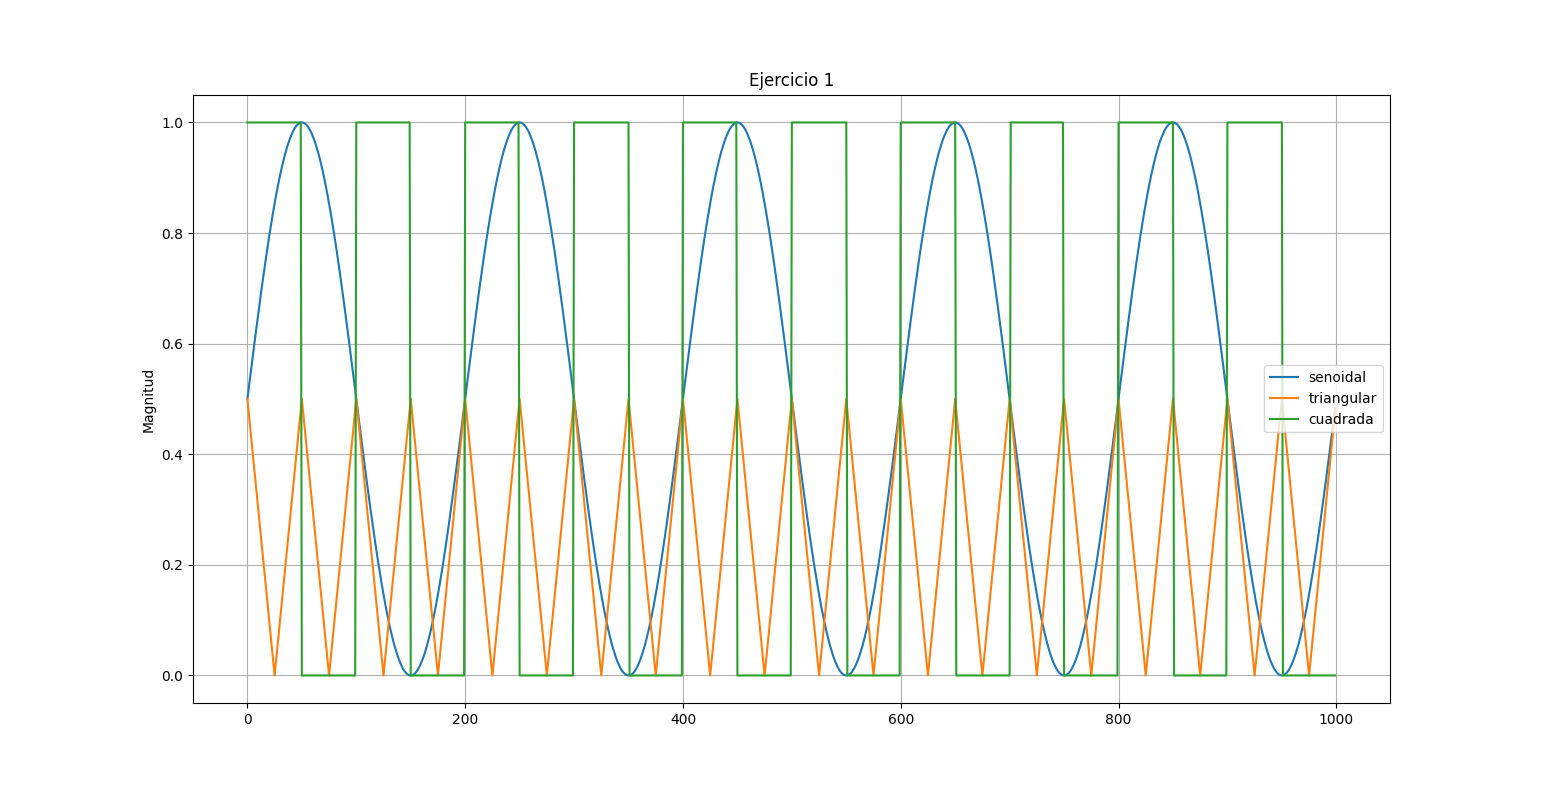
\includegraphics[width=\textwidth]{../img/fig1.png}
	\caption{Demostración del funcionamiento del script.}
	\label{fig:demo}
\end{figure}

El punto 2.1 se puede observar en la figura \ref{fig:nodiff} y no es posible diferenciar las señales.

\begin{figure}[htbp]
	\centering
	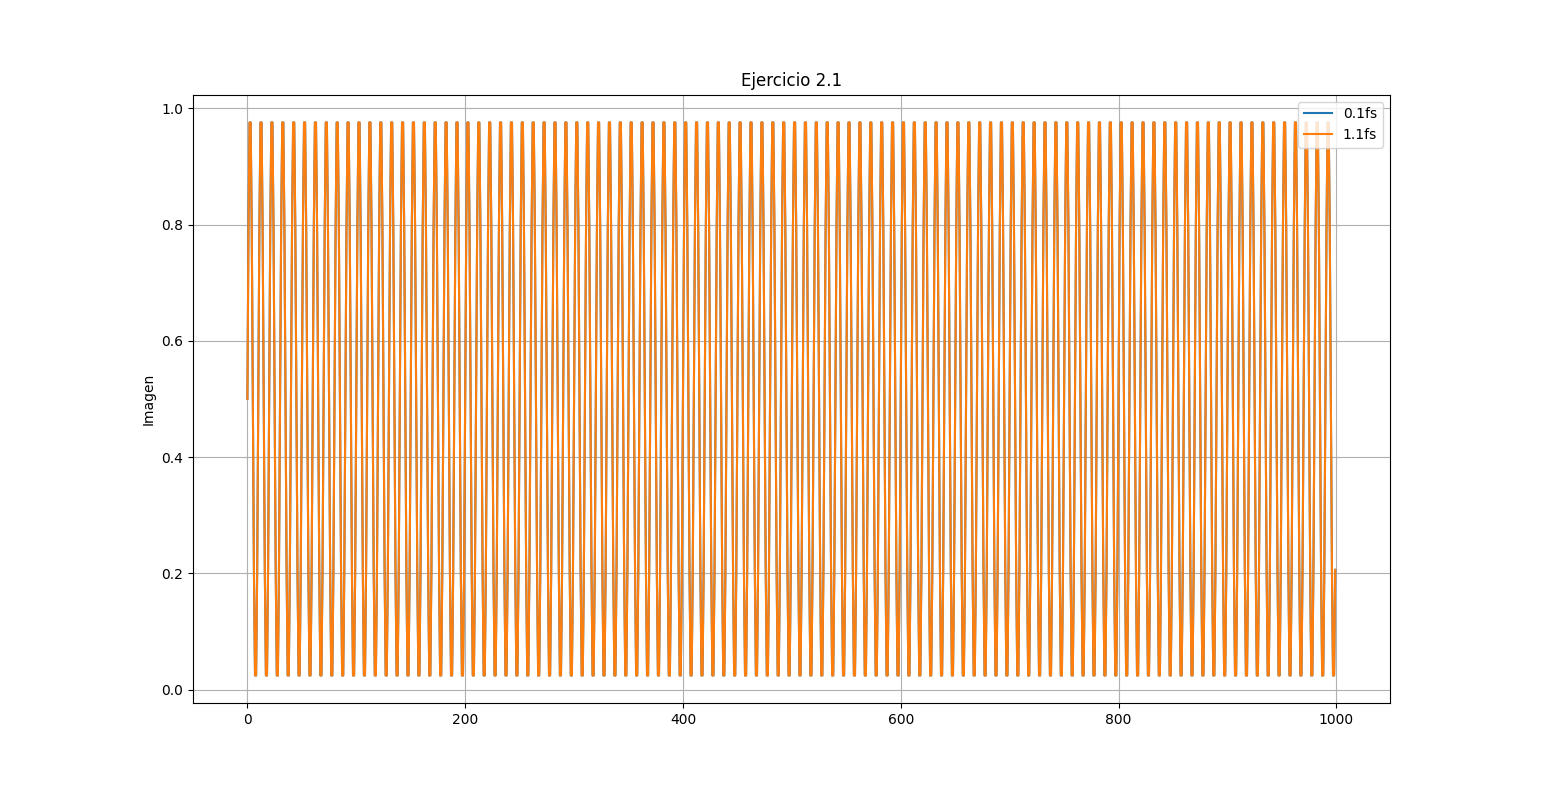
\includegraphics[width=\textwidth]{../img/fig2.png}
	\caption{Ejercicio 2.1.}
	\label{fig:nodiff}
\end{figure}

El punto 2.2 se puede observar en la figura \ref{fig:fase} y es posible apreciar
que aparentan tener la misma frecuencia con una diferencia de fase de 180 grados.

\begin{figure}[htbp]
	\centering
	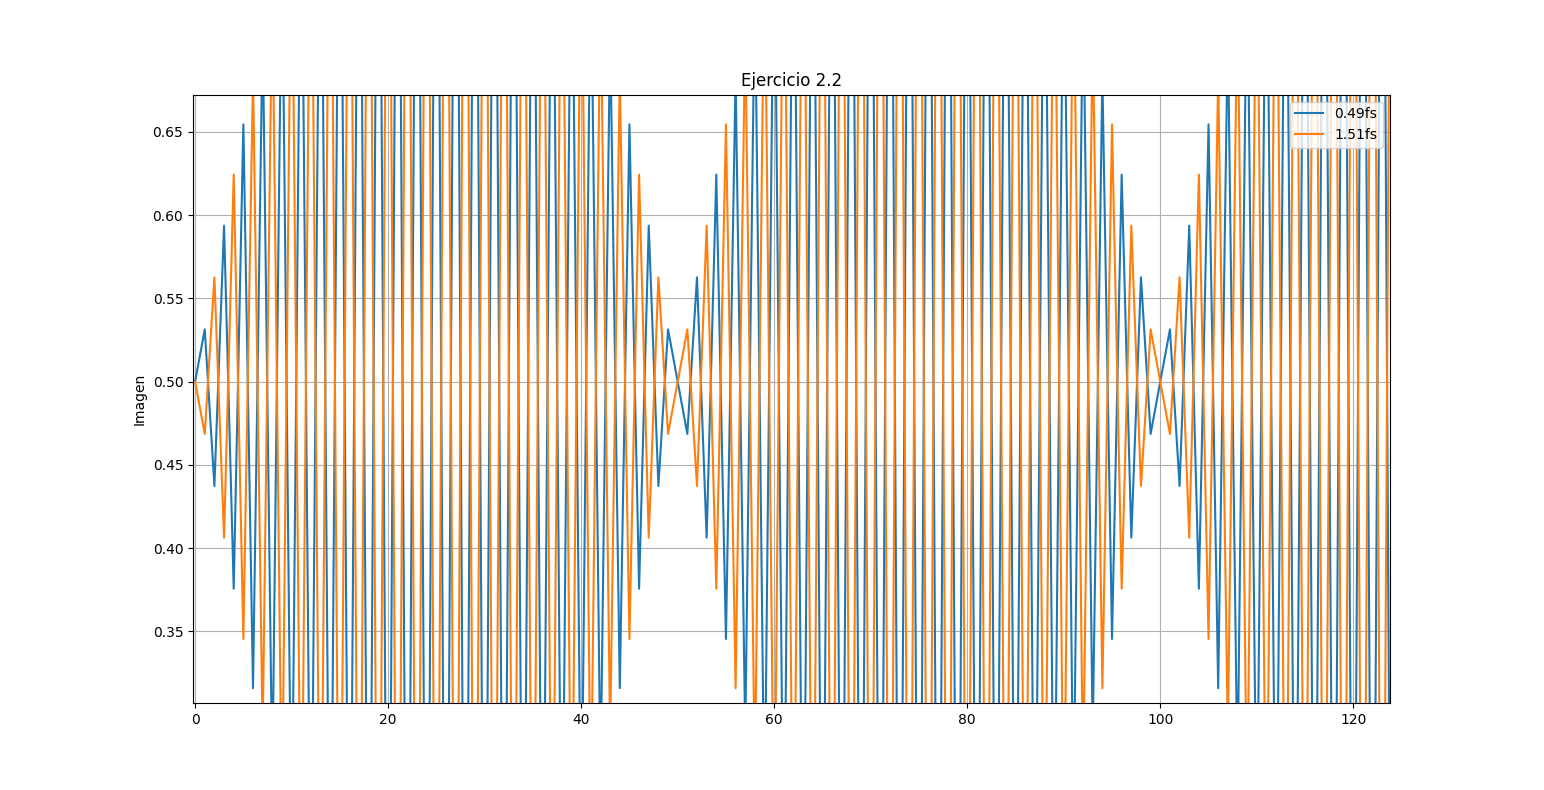
\includegraphics[width=\textwidth]{../img/fig3.png}
	\caption{Ejercicio 2.2.}
	\label{fig:fase}
\end{figure}
\end{document}